\documentclass{article}
\usepackage[minionint,mathlf,textlf]{MinionPro} % To gussy up a bit
\usepackage[margin=1in]{geometry}
\usepackage{graphicx} % For .eps inclusion
%\usepackage{indentfirst} % Controls indentation
\usepackage[compact]{titlesec} % For regulating spacing before section titles
\usepackage{adjustbox} % For vertically-aligned side-by-side minipages
\usepackage{array, mathrsfs, mathrsfs, mhchem, amsmath} % For centering of tabulars with text-wrapping columns
\usepackage{hyperref, chemfig}
\usepackage{subfigure}
\usepackage[autolinebreaks,framed,numbered]{mcode}
\newcommand{\Lapl}{\mathscr{L}}

\pagenumbering{gobble} 
\setlength\parindent{0 cm}
\begin{document}
\large

\section*{Turing patterns}

In our last lecture on regeneration, you saw that the hydra's ``head" is a ring surrounding its ``mouth" on which are found several regularly-spaced tentacles. The number of tentacles is not regular, but depends on the diameter of the regenerating ring on which the tentacles will form. Nonetheless, the tenatcle primordia are appropriately spaced and sized. We likewise find many plants which reliably form leaves (or petals) that are consistent in number but evenly-spaced: the number may vary between sister species, suggesting a labile system for patterning. Alan Turing, whose machines we discussed earlier in the course when evaluating the computational power of biological systems, was inspired by these patterns to describe his now-famous ``chemical basis for morphogenesis," the subject of today's lecture.

\begin{center}
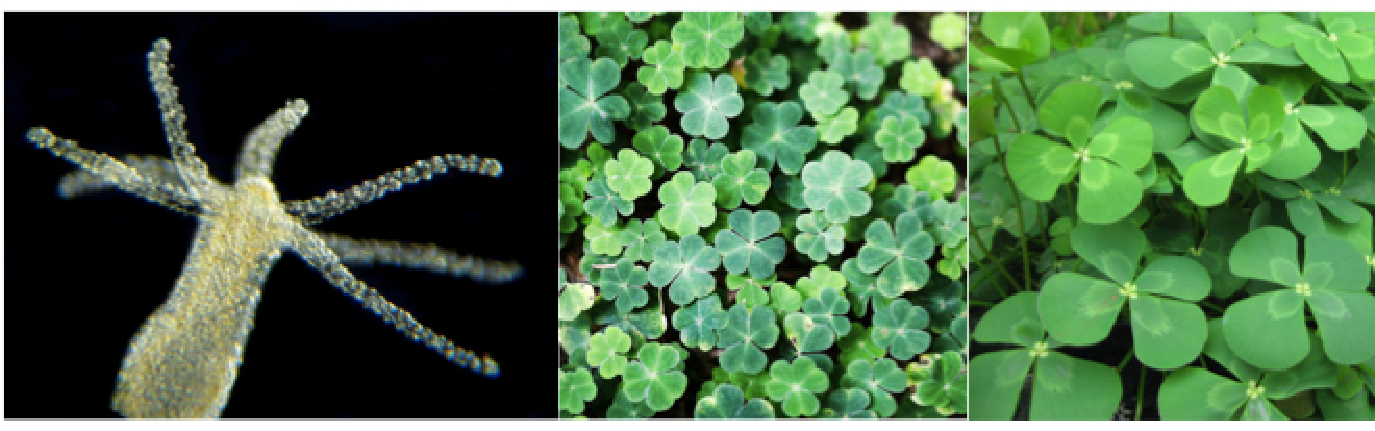
\includegraphics[width=0.7\textwidth]{hydra_leaves.pdf}
\end{center}

In his 1952 paper, Turing coined the term morphogen and described two-morphogen systems diffusing and reacting on rings or spheres. Turing envisioned a very specific type of reaction system: in the absence of diffusion, the concentrations of the two morphogens would approach steady-state values that would be the same across the entire surface (a spatially-homogeneous solution). However, in the presence of diffusion, the same fixed point would become unstable and small chance perturbations from that state would be amplified. Later researchers concerned themselves with how these perturbations could eventually be capped.\\

Bicoid, the first morphogen, was identified only in 1988 by Driever and N\"{u}sslein-Volhard. Since then, the search has been on for morphogen pairs with properties consistent with Turing's model. Most of the patterns which have been shown to be caused by Turing systems are not the quintissential ``spots and stripes." Your tenth and final discussion paper concerns a system for digit patterning: it contains additional detail beyond Turing's essential mechanism, as is usually the case. However, spot and stripe patterning is for the most part still not understood.

\section*{Turing's criteria}

Consider a system of two morphogens, $A$ and $B$, capable of diffusing extracellularly and undergoing reactions which may depend on their own concentrations according to the functions $f$ and $g$:
\[ \frac{\partial }{\partial t} \begin{pmatrix} A(x,t) \\ B(x,t) \end{pmatrix} = \begin{pmatrix} f(A,B) \\ g(A,B) \end{pmatrix} + \begin{pmatrix} D_A & 0 \\ 0 & D_B \end{pmatrix} \frac{\partial^2}{\partial x^2} \begin{pmatrix} A(x,t) \\ B(x,t) \end{pmatrix} \]
For the moment we won't concern ourselves with the identity of the reactions. Instead, we'll look for a type of solution: when $D_A=D_B=0$, the system will be stable and spatially homogeneous, but for appropriately chosen $f$, $g$, and $D_i$, the same fixed point will be unstable. This choice may seem peculiar as we commonly envision diffusion as a ``smoothing" influence on concentration profiles, but as noted for the hydra head organizers above, this is not always the case.\\

The solutions we are looking for will have a fixed point where the concentrations are the same everywhere: we'll call that point $(A^*,B^*)$. Whatever $f$ and $g$ might be, we can linearize our system around this fixed point to determine its stability. Defining the deviations from the fixed point by:
\[ \alpha(x,t) = A(x,t) - A^* \hspace{4 cm} \beta(x,t) = B(x,t) - B^*\]
and defining the Jacobian evaluated at the equilibrium point by some real-valued matrix $\mathbf{C}$:
\[ \mathbf{C} = \begin{pmatrix} \frac{\partial f}{\partial A} & \frac{\partial f}{\partial B}\\ \frac{\partial g}{\partial A} & \frac{\partial g}{\partial B} \end{pmatrix}_{(A^*, B^*)} \]
The system becomes:
\begin{eqnarray}
 \frac{\partial }{\partial t} \begin{pmatrix} \alpha (x,t) \\ \beta (x,t) \end{pmatrix} =  \begin{pmatrix} c_{11} & c_{12} \\ c_{21} & c_{22} \end{pmatrix} \begin{pmatrix} \alpha (x,t) \\ \beta (x,t) \end{pmatrix} + \frac{\partial^2}{\partial x^2} \begin{pmatrix} \alpha (x,t) \\ \beta(x,t) \end{pmatrix} = \mathbf{C}  \begin{pmatrix} \alpha (x,t) \\ \beta (x,t) \end{pmatrix} + \mathbf{D} \frac{\partial^2}{\partial x^2}  \begin{pmatrix} \alpha (x,t) \\ \beta (x,t) \end{pmatrix} \label{eqn:turing}
 \end{eqnarray}
We want solutions where this fixed point is stable if $\mathbf{D}=0$. For that to be true, $\mathbf{C}$ must have two eigenvalues with negative real parts. The eigenvalues of $\mathbf{C}$ are defined as solutions to:
\begin{eqnarray*}
  \mathbf{C} \mathbf{v}_i = \lambda_i \mathbf{v}_i & \implies & \left( \mathbf{C} - \lambda_i \mathbf{I} \right) \mathbf{v}_i = 0\\
  \begin{vmatrix} c_{11} - \lambda_i & c_{12}\\c_{21} & c_{22} - \lambda_i \end{vmatrix} & = & \left(c_{11} - \lambda_i \right)\left(c_{22} - \lambda_i \right) - c_{12} c_{21} =  0\\
  \lambda_i^2 - \left(c_{11} + c_{22} \right) + c_{11}c_{22} - c_{12} c_{21} = 0 & \implies & \lambda_i = \frac{c_{11} + c_{22}  \pm \sqrt{\left(c_{11} + c_{22} \right) ^2 - 4 \left( c_{11}c_{22} - c_{12} c_{21} \right)}}{2}
\end{eqnarray*} 
The pair of eigenvalues will be centered at some point $(c_{11}+c_{22})/2$ and displaced to the left and right of that point according to the value of the discriminant. If $(c_{11}+c_{22})/2 > 0$, then at least one eigenvalue will have positive real part, which is not allowable. Even with $c_{11}+c_{22} < 0$, it would be possible to have one eigenvalue with a positive real part if the discriminant term were very large. Therefore we require $c_{11}c_{22} - c_{12} c_{21} > 0$ so that the discriminant term is smaller than the magnitude of the eigenvalues' mean.\\

To summarize, both eigenvalues have real negative part only if both of the following conditions hold:
\begin{eqnarray}
 \textrm{(i) Tr($\mathbf{C}$) }= c_{11} + c_{22} < 0 \hspace{4 cm} \textrm{(ii) det($\mathbf{C}$) }=  c_{11}c_{22} - c_{12} c_{21} > 0 \label{eqn:conditionsfromstability}
 \end{eqnarray}
These are the conditions for the spatially-homogeneous fixed point to be stable in the absence of diffusion. Now we will determine what additional constraints are set by the requirment that the same fixed point be unstable when diffusion occurs.\\

We will consider a special form for the perturbations about the fixed point $(A^*, B^*)$:
\[  \begin{pmatrix} \alpha (x,t) \\ \beta (x,t) \end{pmatrix} =  \begin{pmatrix} \alpha_0 \\ \beta_0 \end{pmatrix} e^{\lambda t} e^{iqx} \]
In other words, the perturbations are spatial waves whose amplitude is either growing or shrinking in time, depending on the sign of $\lambda$. This form allows us to easily calculate the derivatives and plug them into equation \ref{eqn:turing}:
\begin{eqnarray*}
\lambda \begin{pmatrix} \alpha_0 \\ \beta_0 \end{pmatrix} e^{\lambda t} e^{iqx} & = & \mathbf{C} \begin{pmatrix} \alpha_0 \\ \beta_0 \end{pmatrix} e^{\lambda t} e^{iqx} - q^2 \mathbf{D} \begin{pmatrix} \alpha_0 \\ \beta_0 \end{pmatrix} e^{\lambda t} e^{iqx}\\
\left(  \mathbf{C} -  q^2 \mathbf{D}  - \lambda \mathbf{I} \right) \begin{pmatrix} \alpha_0 \\ \beta_0 \end{pmatrix} & = & 0
\end{eqnarray*}
The fixed point is unstable if at least one of the eigenvalues of the matrix $\mathbf{C} -q^2 \mathbf{D}$ has  positive real part. This is true if either:
\begin{eqnarray*}
\textrm{ Tr($\mathbf{C}  - q^2 \mathbf{D}$) } &= &c_{11} + c_{22} - q^2 \left(D_A + D_B \right) > 0, \textrm{ or }\\
\textrm{ Det($\mathbf{C} - q^2 \mathbf{D}$) } & = & c_{11}c_{22} - c_{12} c_{21}  - q^2 \left( c_{11} D_B + c_{22} D_A \right) + q^4 D_A D_B < 0
\end{eqnarray*}
The first of these inequalities can never be true: from conditions \ref{eqn:conditionsfromstability} we know that $c_{11} + c_{22} < 0$, and $q^2(D_A + D_B)$ is also a positive quantity. Therefore in addition to conditions \ref{eqn:conditionsfromstability}, we require only that:
\begin{eqnarray}
\left| \mathbf{C} - q^2 \mathbf{D} \right| = c_{11}c_{22} - c_{12} c_{21}  - q^2 \left( c_{11} D_B + c_{22} D_A \right) + q^4 D_A D_B < 0 \label{eqn:conditioninstability}
\end{eqnarray}
The only term in this sequence that could be negative is $-q^2(c_{11} D_B + c_{22} D_A)$. If $c_{11}$ and $c_{22}$ are both negative, then condition \ref{eqn:conditioninstability} can never hold. Similarly, if both $c_{11}$ and $c_{22}$ are positive, then condition \ref{eqn:conditionsfromstability} does not hold. Therefore it must be true that $c_{11}$ and $c_{22}$ have opposite sign and $c_{11}c_{22} < 0$. Combining this knowledge with the second condition of \ref{eqn:conditionsfromstability}:
\[ c_{11}c_{22} - c_{12} c_{21} > 0 \implies c_{12} c_{21}  < 0 \]
so $c_{12}$ and $c_{21}$ also have opposite signs. Therefore the signs in the Jacobian $\mathbf{C}$ can take on one of two patterns:
\[ \begin{pmatrix} + & - \\ + & - \end{pmatrix} \hspace{2 cm} \textrm{ or } \hspace{2 cm}  \begin{pmatrix} + & + \\ - & - \end{pmatrix} \]
This concludes the limitations placed solely on the Jacobian (and therefore on our choice of $f$ and $g$). There are also constraints placed on the possible values of the diffusion coefficients for any given $\mathbf{C}$. The left-hand side of inequality \ref{eqn:conditioninstability} is quadratic (in $q^2$) -- the solution to the corresponding equality would therefore  be:
\[ q^2 = \frac{c_{11} D_B + c_{22} D_A \pm \sqrt{\left( c_{11} D_B + c_{22} D_A \right)^2 - 4 \left( c_{11} c_{22} - c_{12} c_{21} \right)D_A D_B }}{2 D_A D_B} \]
The only way for this value to be negative is for the discriminant to be positive:
\[ \left( c_{11} D_B + c_{22} D_A \right)^2 > 4 \left( c_{11} c_{22} - c_{12} c_{21} \right)D_A D_B \]
With some rearrangements, and invoking the signs of $c_{11}$ and $c_{22}$:
\[ \frac{c_{11}}{D_A} - \frac{c_{22}}{D_B} > 2 \sqrt{\left| \frac{c_{12}}{D_A} \right| \left| \frac{c_{21}}{D_B} \right|} > 0 \]
One consequence of this is that:
\[ \frac{c_{11}}{D_A} + \frac{c_{22}}{D_B} > 0 \implies  \frac{c_{11}}{D_A} > \frac{|c_{22}|}{D_B} \]
In other words, the dispersion in $B$ will be greater than the dispersion in $A$.\\

We now have enough information to return to the biological grounding of these solutions. Consider the first possible Jacobian sign pattern mentioned above, which corresponds to an activator-inhibitor pair similar to what was observed for head organizing center patterning in dissociated hydra. Positive fluctuations in $A$ tend to increase the fluctuations of both $A$and $B$. Positive fluctuations in $B$, however, tend to inhibit both $A$ and $B$ itself. If both activator and inhibitor have the same strength, then our condition on dispersion requires that the inhibitor have a greater diffusion coefficient: that is, the activator stays near the source while the inhibitor acts at long ranges.\\

The second Jacobian sign pattern corresponds to the autocatalyzation of formation of a product $A$ from a substrate $B$. Positive fluctuations in both $A$ and $B$ tend to increase the fluctuations in $B$. However, $B$ is consumed by product formation. This type of system is called substrate depletion.\\

\section*{Aside: achieving differences in diffusion coefficients}

In both cases above, the dispersion of the inhibitor must be greater than that of the activator. One way to achieve this would be to have very different diffusion coefficients for the inhibitor and activator. This would be rather easy if the inhibitor were a small molecule and the activator a protein, but otherwise the Stokes-Einstein equation would suggest we should despair:
\[ D = \frac{k_B T}{6 \pi \eta r} \]
where $\eta$ is the viscosity of the medium and $r$ is the effective radius of the (presumed globular) molecule. We would need to make a protein about 1000 times as long as usual in order to increase its effective radius by a factor of ten. However, diffusible, proteinaceous activator-inhibitor pairs are often found in nature and it is observed empircally that their diffusion coefficients may differ significantly.\\

Receptor binding impedes movement (as does nuclear retention in diffusion through syncytia) and can explain the lower diffusion coefficients of the activator. To see why this works, consider an activator $A$ and inhibitor $B$ which diffuse at the same rate, but the activator is involved in a binding reaction to an immobile receptor $R$:
\begin{eqnarray*}
\frac{d[A]}{dt} & = & f([A],[B]) + D \frac{\partial^2 [A]}{\partial x^2} - k_1 [A] [R] + k_{-1} [AR]\\
\frac{d[B]}{dt} & = & g([A], [B]) + D \frac{\partial^2 [B]}{\partial x^2}\\
\frac{d[AR]}{dt} & = & k_1 [A] [R] - k_{-1} [AR] \\
\end{eqnarray*}
If the free receptor is bountiful so that $[R]\approx r_0$ is effectively constant, and if $k_1, k_{-1}$ are large enough that receptor binding is in rapid equilibrium, then
\[ \frac{d[AR]}{dt} = \frac{r_0 k_1}{k_{-1}} \frac{d[A]}{dt} = k \frac{d[A]}{dt} \]
Then we can add the first and third differential equations together to obtain:
\[ \left( 1 + k \right) \frac{d[A]}{dt} = f([A],[B]) + D \frac{\partial^2 [A]}{\partial x^2} \]
Thus for sufficiently large receptor concentrations or appropriate binding rates, the effective diffusion coefficient of $A$, $D/(1+k)$, may be much smaller than the unaffected diffusion coefficient of $B$\footnote{As Michael mentioned during the regeneration lecture, diffusible inhibitors must have a mechanism of action, and typically this is either that they bind to the activator itself or that they bind to the activator's receptor.  The latter would tend to inhibit diffusion of $B$ as well: however, note that this type of inhibitor does not have the properties required for Turing patterning.}.

\section*{Finite field length}

Another grounding consideration is that the field of cells undergoing patterning will not be infinite. The only possible solutions on a finite field of length $L$ are combinations of waves with discrete values given by the wave numbers $q_n$:
\[ \begin{pmatrix} \alpha(x,t) \\ \beta(x,t) \end{pmatrix} = \sum_n  \begin{pmatrix} \alpha_{0,n} \\ \beta_{0,n} \end{pmatrix} e^{\lambda_n t} e^{iq_n x}, \hspace{2 cm} q_n = \frac{2 \pi n}{L}  \]
Any given mode of this solution will be unstable in the presence of diffusion only if condition \ref{eqn:conditioninstability} holds for its value $q_n$, i.e.
\[ \left| \mathbf{C} - q_n^2 \mathbf{D} \right| = c_{11}c_{22} - c_{12} c_{21}  - q_n^2 \left( c_{11} D_B + c_{22} D_A \right) + q_n^4 D_A D_B < 0 \]
In the right half plane, the left-hand side of this inequality crosses the $x$ axis twice: in between, it is less than zero. The whole numbers $n$ whose corresponding $q_n$ falls in this region represent unstable nodes. As $L$ changes, so will the number and identity of the nodes within the region.\\

For a very small organism, there may be no unstable modes at all. A slightly large organism might have only one or two unstable mode (picture a guinea pig), while a very large organism might have spots (if diffusion is equal in both dimensions) or stripes. Similarly, if a field of cells is larger in one dimension than the other, it might only be possible to form stripes perpendicular to the longer dimension, as in the simulations of tapered tails below. The dependence of pattern on field size could explain, for example, why the number of stripes on a fish increases as it grows. It may also suggest the origin of developmental patterning errors such as supernumerary digits.

\begin{center}
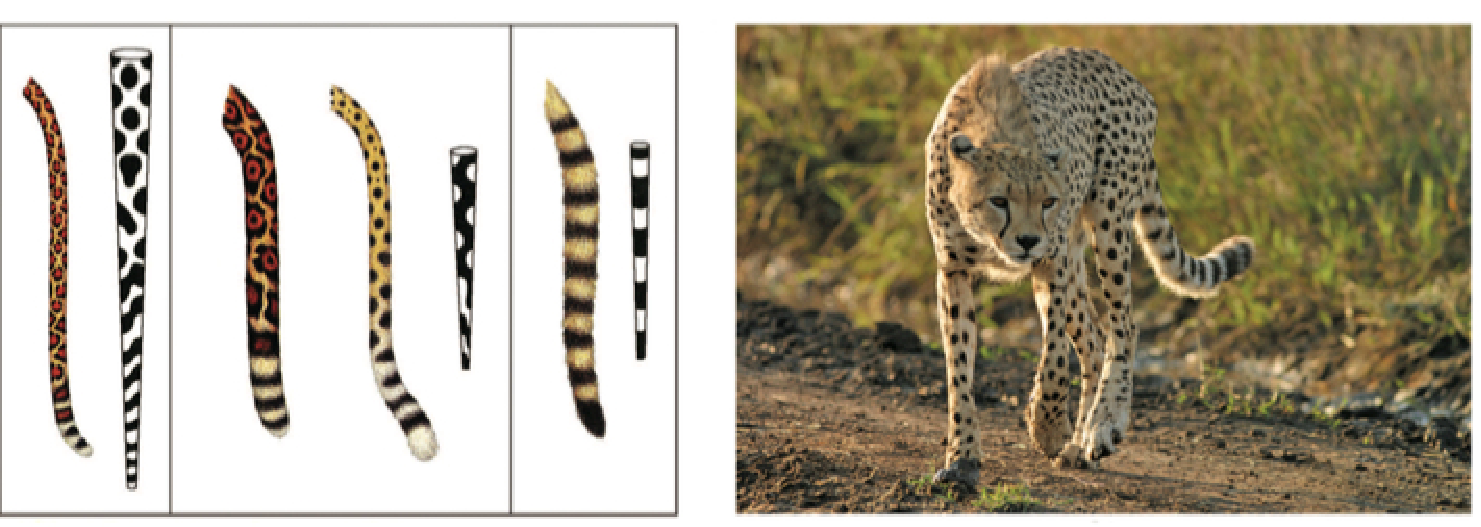
\includegraphics[width=0.8\textwidth]{tail.pdf}
\end{center}


\section*{Gierer and Meinhardt (1972)}

Now that we know the requirements on $c_{ij}$ and $D_i$, we could easily define a linear reaction system with the properties we require:
\begin{eqnarray*}
 \frac{\partial }{\partial t} \begin{pmatrix} A (x,t) \\ B (x,t) \end{pmatrix} =  \begin{pmatrix} c_{11} & c_{12} \\ c_{21} & c_{22} \end{pmatrix} \begin{pmatrix} A (x,t) \\ B (x,t) \end{pmatrix} + \frac{\partial^2}{\partial x^2} \begin{pmatrix} A (x,t) \\ B (x,t) \end{pmatrix} 
 \end{eqnarray*}
This low-hanging fruit is rotten, however, beoncause we know the system is unstable, and this system implies unrealistically that concentrations will go off to infinity. The trick is to choose reaction terms in such a way that the Jacobian has the properties we want but the concentrations are naturally bounded.\\

Many such reaction terms have been previously described. One of the most famous is the activator-inhibitor systems elaborated by Gierer and Meinhardt in 1972, one of which is:
\[ \frac{\partial A}{\partial t} = k_1 - k_2 A + \frac{k_3 A^2}{B^4} + D_A \frac{\partial^2 A}{\partial x^2} \hspace{ 2 cm}  \frac{\partial B}{\partial t} = - k_2 B + \frac{k_4 A^2}{B^4} + D_B \frac{\partial^2 B}{\partial x^2} \]
%\[ \frac{\partial A}{\partial t} = \frac{k_1 A^2}{B} - k_2 A + D \frac{\partial^2 A}{\partial x^2} \hspace{ 2 cm}  \frac{\partial B}{\partial t} = k_1 A^2 - k_2 B + (D+\varepsilon) \frac{\partial^2 B}{\partial x^2} \]
Here, we imagine that $A$ functions as a dimer (explaining why the $A$-dependent production terms $\sim A^2$) and that $B$ is an inhibitor with a higher Hill coefficient.


\section*{Daniel Thomas (1975)}
So far we have focused on systems where the activator ``A" is a signaling protein and ``B" is its inhibitor, assumed to act by binding to ``A". Now we consider a system where ``A" and ``B" might as easily be small molecules:
\begin{eqnarray*}
\frac{\partial A}{\partial t} & = & \gamma \left[ A_0 - A - \rho \, h(A,B) \right] + \frac{\partial^2 A}{\partial x^2}\\
\frac{\partial B}{\partial t} & = & \gamma \left[ \alpha \left(  B_0 - B \right) - h(A,B) \right] + \beta \frac{\partial^2 B}{\partial x^2} \\
h(A,B) & = & \frac{ A \, B}{1 + A + K A^2} 
\end{eqnarray*}
In addition to the normal production and degradation terms, we have a degradation term of the following form (non-dimensionalization of the equations above has simplified the denominator):
\[ \left[ B \right] \left( \frac{\left[ A \right]/K_1}{1 + \left[ A \right]/K_1} \right)\left( \frac{1}{1 + \left[ A \right]/K_2} \right) \]
This form of reaction rate has been empirically observed for, e.g., uric acid oxidation by uricase (Murray 1988). We might think of $A$ and $B$ in this case as two substrates for an enzyme that will catalyze a reaction consuming both of them. $[B]$ always remains small enough to stay within the first-order regime, but the reaction follows Michaelis-Menten kinetics for $[A]$ $\ldots$ up to a point. When $[A]$ is very large, $A$ becomes an inhibitor of the reaction.\\

For these reaction terms,
\[ \mathbf{C} = \begin{pmatrix} -1 - \frac{k_4 - k_4 k_5 A^2}{(1 + A + k_5 A)^2} &  - \frac{k_4 \, A}{1 + A + k_5 \, A} \\  - \frac{k_4 - k_4 k_5 A^2}{(1 + A + k_5 A)^2} & - k_3 - \frac{k_4 \, A}{1 + A + k_5 \, A} \end{pmatrix}_{(A^*,B^*)} \]
Without having explicitly calculated the spatially-homogeneous fixed point $(A^*,B^*)$, we know already that if this system is to function as a Turing pattern, the only possible sign pattern is the one corresponding to the activator-inhibitor system. In other words, $B$ is functioning as the inhibitor of $A$ by facilitating its enzymatic degradation.\\

J.D. Murray (1981) produced an iconic diagram showing the variety of patterns that can arise from this model with only $\gamma$ variable. The significance of this is that it scales the relative magnitude of reaction vs. diffusion terms.

\begin{center}
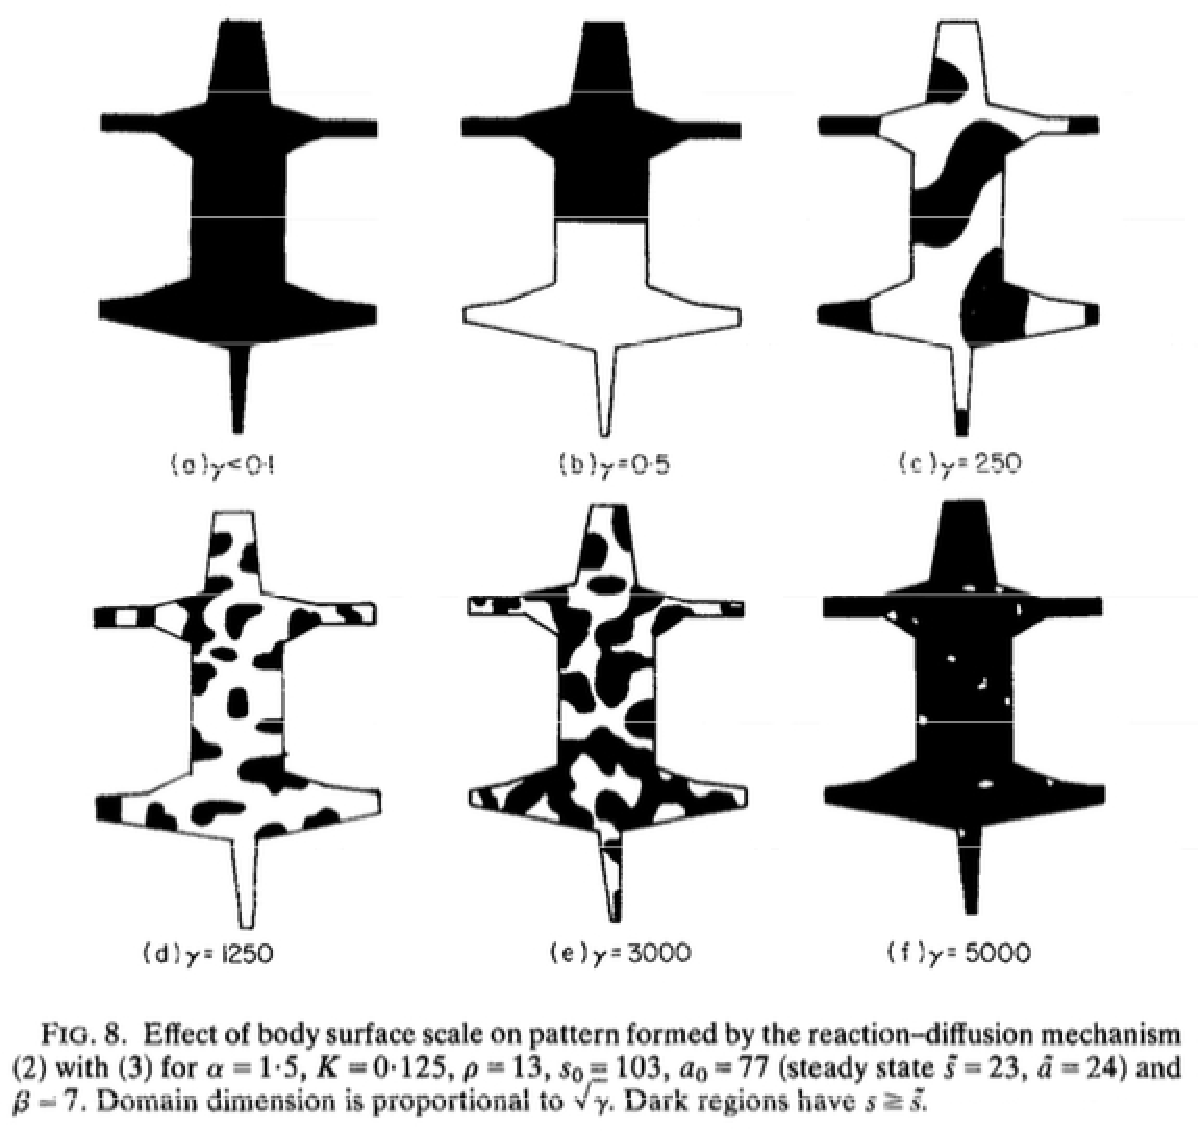
\includegraphics[width=0.7\textwidth]{thomas_murray.pdf}
\end{center}

\section*{Substrate depletion: Schnakenberg model}

The Schnakenberg model has three main reactions:
\[ \ce{A <=>[k_2][k_1] \varnothing } \hspace{3 cm} \ce{\varnothing {\color{white}.} ->[k_3] B} \hspace{3 cm} \ce{2A + B ->[k_4] 3 A} \]
In other words, we have a somewhat implausible three-molecule reaction converting $B$ to $A$, and no other degradation term for B. 
Using the law of mass action:
\[ f(A,B) = k_1  - k_2 A + k_4 A^2 B \hspace{2 cm} g(A,B) = k_3 - k_4 A^2 B \]
If this system behaves like a Turing pattern, then the only possible sign pattern for the reaction Jacobian is the one corresponding to substrate depletion. We can understand this from the reactions proposed: $A$ autocatalyzes its own production but this process requires a substrate, $B$, which can be depleted.\\

It is possible to non-dimensionalize this system and solve for the steady-state:
\[ \frac{\partial A}{\partial t} = \gamma \left( a  - A + A^2 B \right) + \frac{\partial^2 A}{\partial x^2} \hspace{1 cm} \frac{\partial B}{\partial t} = \gamma \left( b -  A^2 B \right) + d \frac{\partial^2 B}{\partial x^2}\]

The fixed for this system is:
\[ (A^*, B^*) = \left( a + b, \frac{b}{(a+b)^2} \right) \]
A simulation of this model on the plane is included below (adapted from the Brooks PDF uploaded to the course website, which outlines a range of parameters with interesting phenomena).  The system is initiated near its fixed point but with small Gaussian fluctuations. Updates occur via Euler's method. The diffusion term is updated to
\[ \frac{\partial A}{\partial t} = \gamma \left( a  - A + A^2 B \right) + \nabla^2 A \hspace{1 cm} \frac{\partial B}{\partial t} = \gamma \left( b -  A^2 B \right) + d \nabla^2 B\]
where $\nabla^2 = \frac{\partial^2}{\partial x^2} + \frac{\partial^2}{\partial y^2}$ is the Laplace operator on the Cartesian plane. These second derivatives are calculated according to the finite difference method:
\[ \nabla^2 f \approx \frac{f(x+h, y) + f(x-h,y) + f(x,y+h) + f(x,y-h) - 4 f(x,y)}{h^2} \]

\begin{lstlisting}
function [] = turing()
    % Create a square mesh of points for the reaction-diffusion system
    N = 30;
    [xx,yy] = meshgrid([0:N], [0:N]);
    
    % Determine how long the simulation will run and how frequently it will
    % update.
    dt = .01/N^2;
    t = 0;
    t_end = 1;
    
    % System parameters for spots (see Brooks PDF for interesting alternatives)
    a = 0.05;
    b = 1;
    d = 20;
    gamma = 600;
    
    % Initiate the system near the spatially-homogeneous fixed point, but with small added noise
    A = (a+b)*ones(size(xx)) + .1*randn(size(xx)); 
    B = (b/(a+b)^2)*ones(size(xx)) + .1*randn(size(xx));
    
    for n = 1:round(t_end/dt)
        t = t+dt;
        
        % Calculate the discrete Laplacian using the finite difference
        % method. Take special care at the edges to allow continuity of
        % diffusion from one edge of the grid to the opposite edge.
        % (Treats the surface as toroidal.)
        AE = A(:,[2:N+1 1]);
        AW = A(:,[N+1 1:N]);
        AN = A([N+1 1:N],:);
        AS = A([2:N+1 1],:);
        BE = B(:,[2:N+1 1]);
        BW = B(:,[N+1 1:N]);
        BN = B([N+1 1:N],:);
        BS = B([2:N+1 1],:);
        A2B = A.^2.*B;
        A = A + gamma*dt*(a - A + A2B) + dt*(AE+AW+AN+AS-4*A)*N^2;
        B = B + gamma*dt*(b - A2B) + d*dt*(BE+BW+BN+BS-4*B)*N^2;
    end
    
    % Display the image
    Ascaled = (A - min(min(A))) ./ (max(max(A)) - min(min(A)));
    imshow(A)
end
\end{lstlisting}

\section*{Caveats}

Not everything that looks promisingly like a Turing pattern is produced by this mechanism. For example, in stripe development in some zebrafish, stripes are formed through melanic cell migration.

\begin{center}
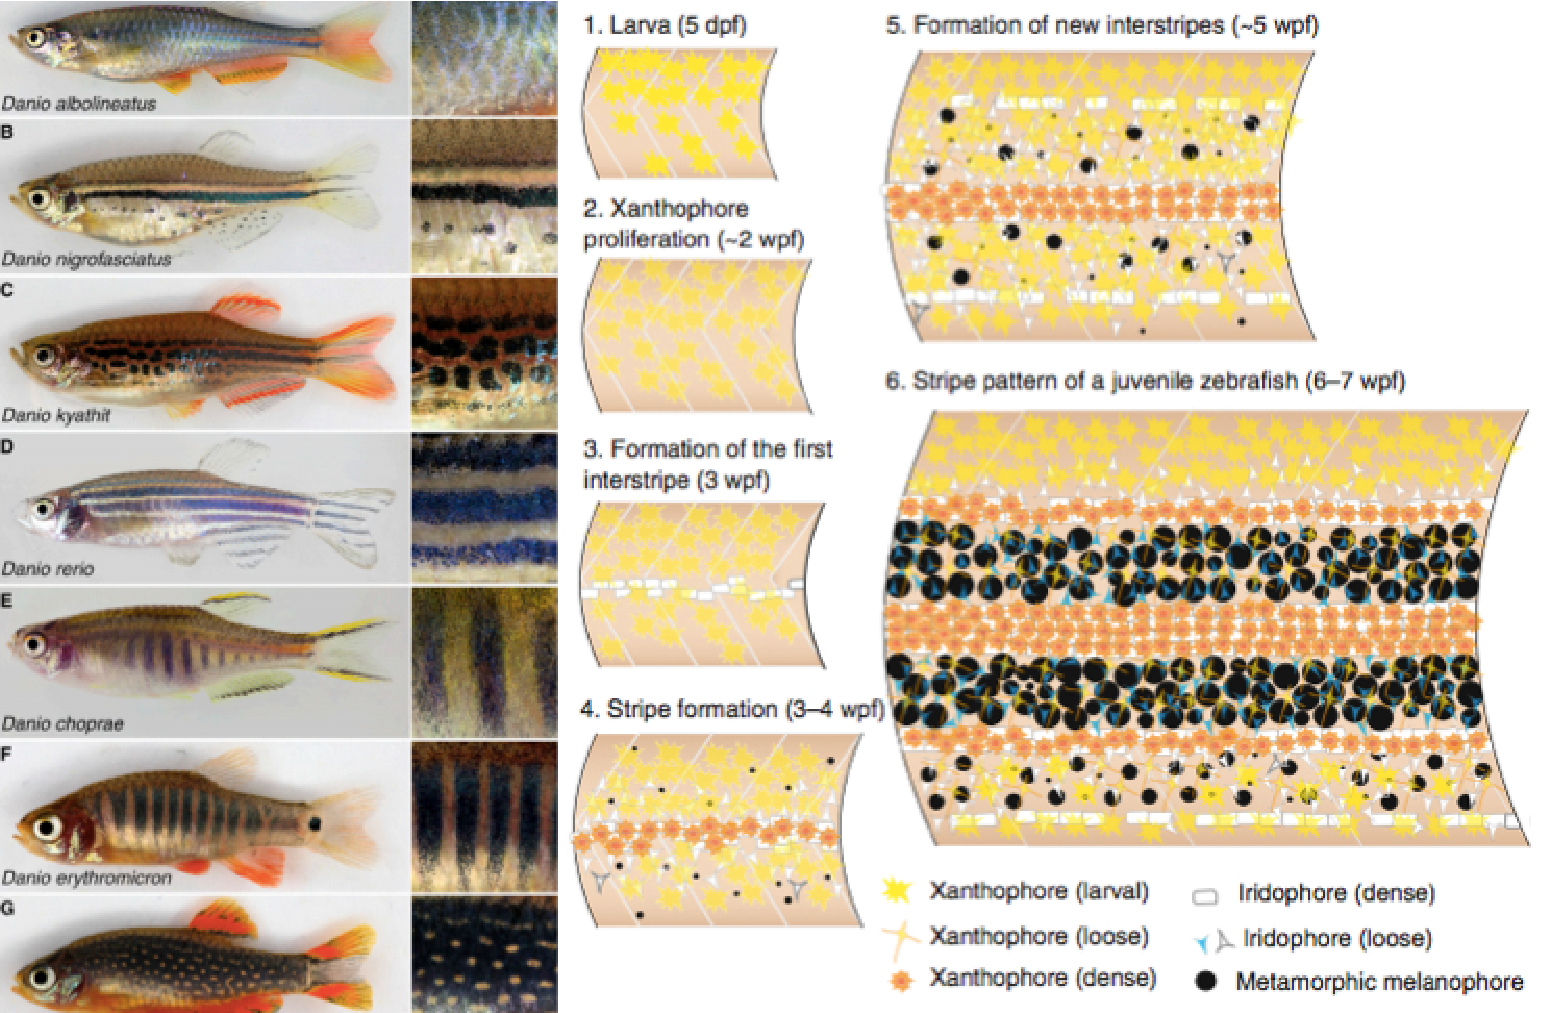
\includegraphics[width=0.7\textwidth]{fish.pdf}
\end{center}

Similarly, the positions of stripes of pair rule gene expression are ``hard-coded" in the fruit fly.

\begin{center}
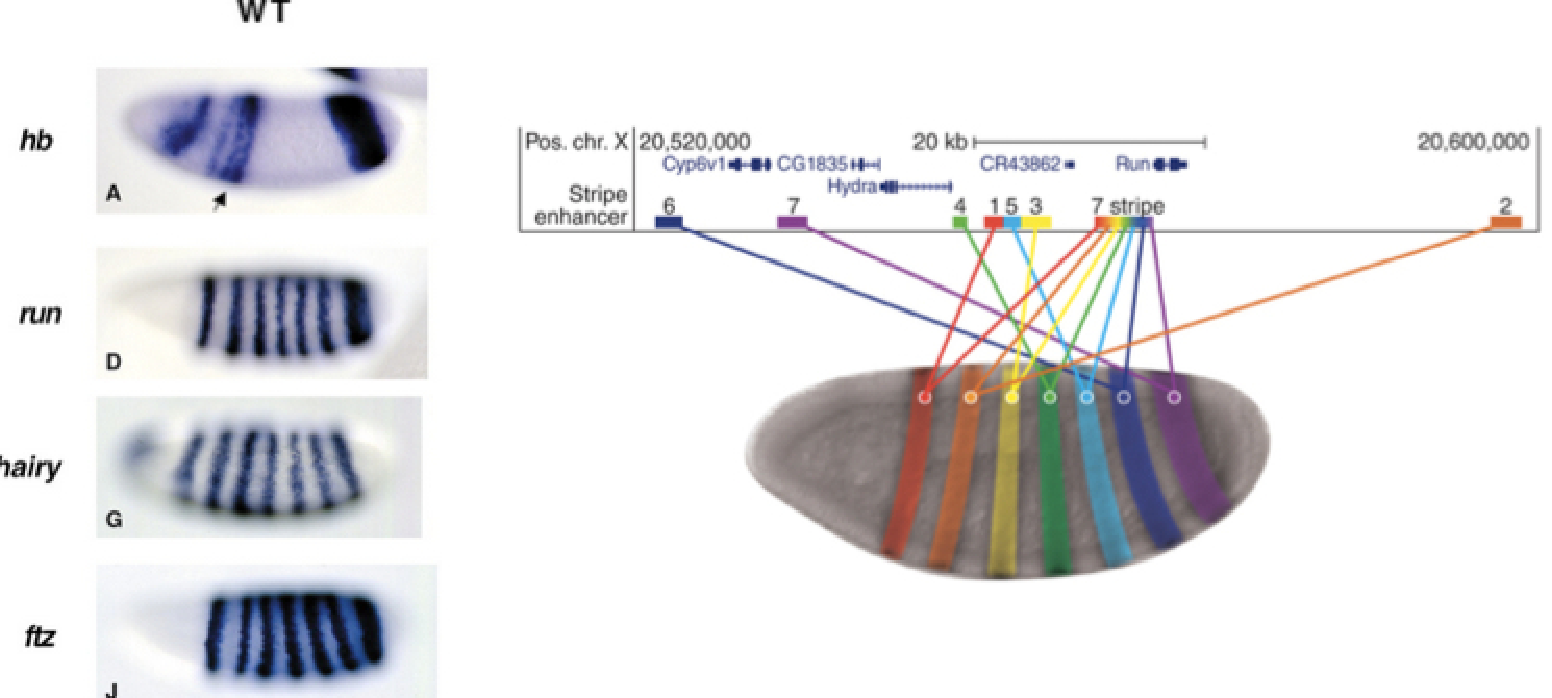
\includegraphics[width=0.7\textwidth]{pairrule.pdf}
\end{center}

\end{document}